\paragraph{Caso d'uso UC 4.3.1: Pubblicazione della lista.}
\label{Caso d'uso UC 4.3.1: Pubblicazione della lista.}

\begin{figure}[ht]
	\centering
	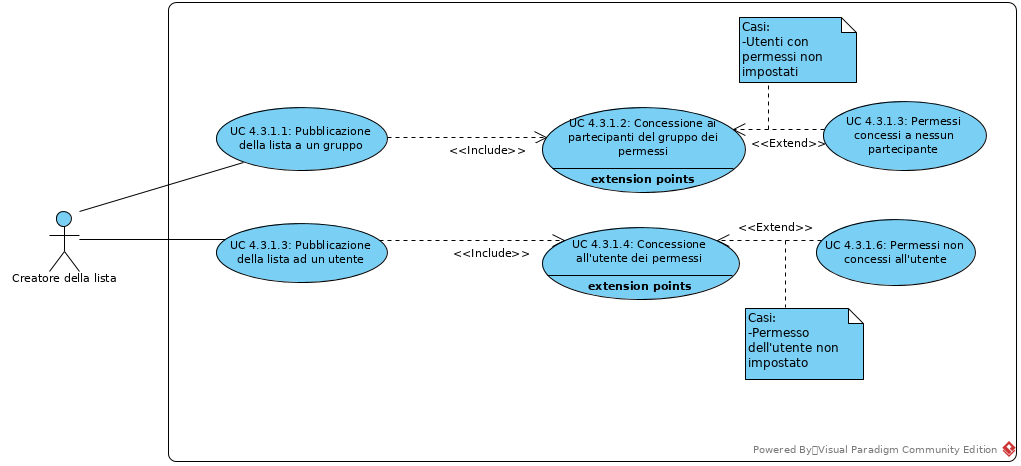
\includegraphics[scale=0.60]{Usecases/img/UC4.3.1.png}
	\caption{Caso d'uso UC 4.3.1: Pubblicazione della lista.}
\end{figure}

\FloatBarrier
\begin{itemize}
\item \textbf{Attori:} Creatore della lista.
\item \textbf{Descrizione:} Il Creatore della lista vuole pubblicare la bolla lista-spesa creata e può farlo in due modi:
\begin{itemize}
\item Pubblicando la bolla lista-spesa a un gruppo.
\item Pubblicando la bolla lista-spesa ad un utente.
\end{itemize}
\item \textbf{Precondizione:} Il Creatore della lista vuole pubblicare la bolla lista-spesa creata. 
\item \textbf{Postcondizione:} Il Creatore della lista ha pubblicato la bolla lista-spesa creata.
\item \textbf{Scenario principale:}
	\begin{itemize}
	\item{Pubblicazione della lista a un gruppo (UC 4.3.1.1).}
	\item{Pubblicazione della lista ad un utente (UC 4.3.1.4).}
	\end{itemize}
\end{itemize}